\chapter{Projekterstellung}\label{chap:Projekterstellung}

\section{Überprüfung Speicherplatz MC-Karte}\label{subsec:Überprüfung Speicherplatz MC-Karte}

Es ist so früh wie möglich zu prüfen, ob die eingesetzte Speicherkarte der CPU groß genug ist, um das Programm und weitere Informationen (z.B. Textlisten) laden zu können. Es sollten Speicherkarten mit mindestens 256MB Speicherkapazität eingesetzt werden.

\clearpage
\section{Anlegen eines Projekts mit Hilfe der Bibliothek}\label{subsec:Anlegen eines Projekts mit Hilfe der Bibliothek}

In diesem Kapitel werden die einzelnen Schritte erklärt, wie in kurzer Zeit ein funktionierendes Gerüst (Hardware, Software) mit Hilfe unserer Bibliothek erstellt werden kann.
Die tieferen Zusammenhänge werden ab Kapitel 9:Hardwarekonfiguration \textbf{TODO!}erläutert.

\begin{enumerate}
    \item Projekt anlegen.
    \begin{figure}[!ht]
        \centering
        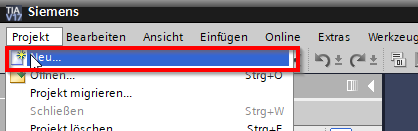
\includegraphics[width = 0.5 \textwidth]{Neues Projekt anlegen.png}
        \caption{Neues Projekt anlegen}
        \label{fig:Neues Projekt anlegen}
    \end{figure}

    \item Bausteinhilfe und S120-Skripte importieren:\par
    \noindent Den Ordner \glqq UserFiles\grqq{} aus der Bibliothek über den File-Explorer in den Projektordner kopieren:
    \begin{figure}[!ht]
        \centering
        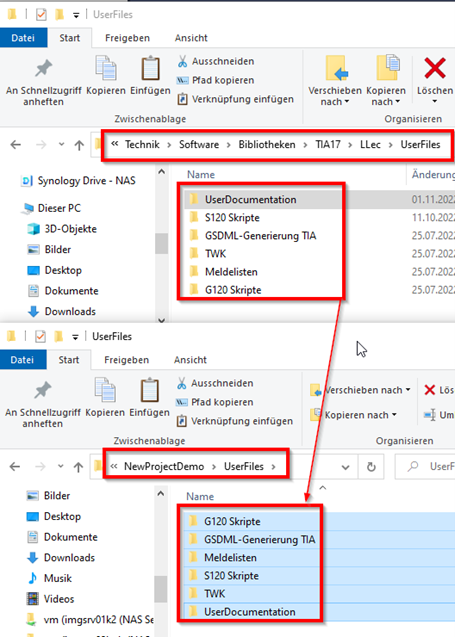
\includegraphics[width = 0.5 \textwidth]{Bausteinhilfe und S120-Skripte in Projektordner kopieren.png}
        \caption{Bausteinhilfe und S120-Skripte in Projektordner kopieren}
        \label{fig:Bausteinhilfe und S120-Skripte in Projektordner kopieren}
    \end{figure}

    \item Rechtsklick auf den Projektnamen im Projektbaum -> Eigenschaften -> Reiter Schutz -> \glqq Beim Übersetzen von Bausteinen Simulierbarkeit unterstützen\grqq{} aktivieren
    \begin{figure}[!ht]
        \centering
        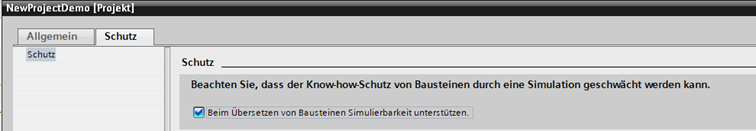
\includegraphics[width = 0.8 \textwidth]{Einstellung Unterstützung Simulierbarkeit von Know-How-geschützen Bausteinen.png}
        \caption{Einstellung Unterstützung Simulierbarkeit von Know-How-geschützen Bausteinen}
        \label{fig:Einstellung Unterstützung Simulierbarkeit von Know-How-geschützen Bausteinen}
    \end{figure}

    \item Ordner \glqq Sprachen \& Ressourcen\grqq{} -> Projektsprachen -> Englisch (USA) aktivieren und als Referenzsprache einstellen. Die Editiersprache entsprechend des Ziellandes / Kundenvorgaben etc. einstellen.
    \begin{figure}[!ht]
        \centering
        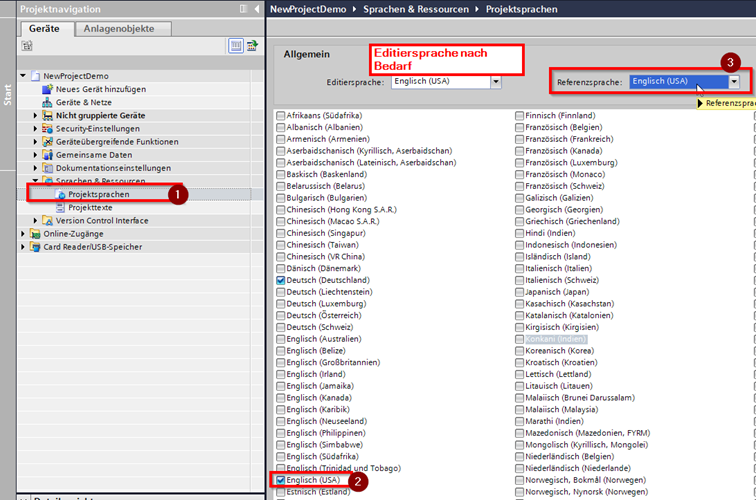
\includegraphics[width = 0.8 \textwidth]{Einstellung der Projektsprachen.png}
        \caption{Einstellung der Projektsprachen}
        \label{fig:Einstellung der Projektsprachen}
    \end{figure}
\clearpage
    \item Bibliothek LLec öffnen. Sollte diese noch nicht im Baum auftauchen, diese entsprechend Anleitung (Kapitel 7.4) \textbf{TODO!} einbinden.
    \begin{figure}[!ht]
        \centering
        \includegraphics[width = 0.35 \textwidth]{Öffnen der Bibliothek.png}
        \caption{Öffnen der Bibliothek}
        \label{fig:Öffnen der Bibliothek}
    \end{figure}

    \item Per Drag’n’Drop aus den Unterordnern Typen und Kopiervorlagen jeweils den gesamten Inhalt in die Projektbibliothek kopieren:
    \begin{figure}[!ht]
        \centering
        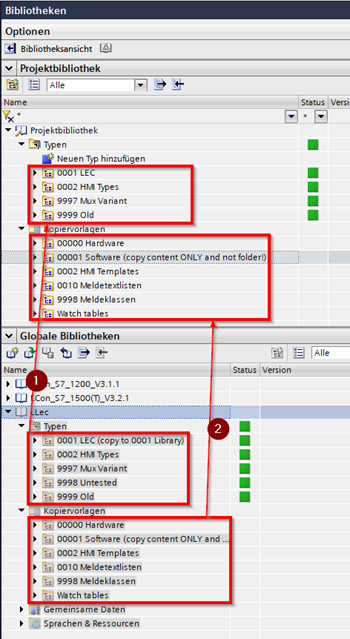
\includegraphics[width = 0.4 \textwidth]{Globale Bibliothek in das Projekt importieren.png}
        \caption{Globale Bibliothek in das Projekt importieren}
        \label{fig:Globale Bibliothek in das Projekt importieren}
    \end{figure}
\clearpage
    \item Meldeklassen aus den Kopiervorlagen in die Meldeklassen unter gemeinsame Dateien im Projekt kopieren. 
    \begin{figure}[!ht]
        \centering
        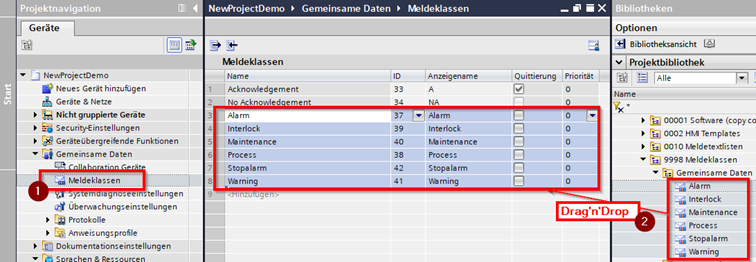
\includegraphics[width = 0.8 \textwidth]{Import der Meldeklassen (Gemeinsame Daten).png}
        \caption{Import der Meldeklassen (Gemeinsame Daten)}
        \label{fig:Import der Meldeklassen (Gemeinsame Daten)}
    \end{figure}

    \item CPU importieren. Dadurch wird automatisch auch das Netz „Processnet“ mit angelegt und verbuden.
    \begin{figure}[!ht]
        \centering
        \includegraphics[width = 0.8 \textwidth]{CPU und Netze einfügen und verbinden.png}
        \caption{CPU und Netze einfügen und verbinden}
        \label{fig:CPU und Netze einfügen und verbinden}
    \end{figure}
    \textcolor{red}{\textbf{ACHTUNG: SPS Name seit TIA V17 geändert!}}



\end{enumerate}